\documentclass{article}
\usepackage{fancyhdr}
\usepackage{lipsum}  
\usepackage{listings} 
\usepackage{xcolor}   
\usepackage{amsmath}
\usepackage{enumitem}
\usepackage{graphicx}
\usepackage{caption}
\usepackage{verbatim}

% Define macros for title and author
\newcommand{\thetitle}{STAT 641 \\ Homework 4}
\newcommand{\theauthor}{Keegan Smith}

\title{\thetitle}
\author{\theauthor}

\pagestyle{fancy}
\fancyhf{}  % Clear all header and footer fields
\fancyhead[L]{\nouppercase{\rightmark}}
\fancyhead[C]{\thetitle}  % Title in the center
\fancyhead[R]{\theauthor}  % Your name on the right

\lstset{ %
  backgroundcolor=\color{lightgray},   % choose the background color
  basicstyle=\ttfamily\small,          % size of fonts used for the code
  keywordstyle=\color{blue},           % color for keywords
  commentstyle=\color{green},          % color for comments
  stringstyle=\color{red},             % color for strings
  numbers=left,                        % where to put the line-numbers
  numberstyle=\tiny\color{gray},       % style for line-numbers
  stepnumber=1,                        % the step between two line-numbers
  numbersep=5pt,                       % how far the line-numbers are from the code
  frame=single,                        % adds a frame around the code
  rulecolor=\color{black},             % frame color
  breaklines=true,                     % automatic line breaking
  breakatwhitespace=false,             % automatic breaks should only happen at whitespace
  showspaces=false,                    % don't show spaces in the code
  showstringspaces=false,              % don't show spaces in strings
  showtabs=false,                      % don't show tabs in the code
}

\begin{document}

\maketitle
\section*{Problem 1}
\begin{enumerate}
\item the likelihood function is: \\
\[
L(\theta_1, \theta_2, \ldots, \theta_k;y) = \Pi_{i=1}^nf(y_i; \theta)
\]
So plugging in the poisson distribution and our data we have: \\
\begin{align*}
L(\theta_1, \theta_2, \ldots, \theta_k;y) &= \Pi_{i=1}^n\frac{\lambda^{y_i}e^{-\lambda}}{y_i!} \\
&= \frac{\lambda^{0}e^{-\lambda}}{0!} \cdot \frac{\lambda^{1}e^{-\lambda}}{1!} \cdot (\frac{\lambda^{2}e^{-\lambda}}{2!})^2 \cdot \frac{\lambda^{3}e^{-\lambda}}{3!} \cdot \frac{\lambda^{4}e^{-\lambda}}{4!} \cdot \frac{\lambda^{5}e^{-\lambda}}{5!} \\
&= e^{-\lambda} \cdot \lambda e^{-\lambda} \cdot \frac{\lambda^{4}e^{-2\lambda}}{4} \cdot \frac{\lambda^{3}e^{-\lambda}}{3!} \cdot \frac{\lambda^{4}e^{-\lambda}}{4!} \cdot \frac{\lambda^{5}e^{-\lambda}}{5!} \\
&= \frac{\lambda^{17} \cdot e^{-7 \lambda}}{69120}
\end{align*}
\item The log likelihood is simply taking the natural log of the likelihood function, so we have: \\
\begin{align*}
\ln (L(\theta_1, \theta_2, \ldots, \theta_k;y)) &= \ln(\frac{\lambda^{17} \cdot e^{-7 \lambda}}{69120}) \\
&= \ln(\lambda^{17}) + \ln(e^{-7\lambda}) - \ln(69120) \\
&= \ln(\lambda^{17}) - 7\lambda - \ln(69120)
\end{align*}
\item The derivative of the log likelihood is as follows: \\
\begin{align*}
\frac{d}{d\lambda}(\ln(\lambda^{17}) - 7\lambda - \ln(69120)) &= 17 \cdot \lambda^{16} \cdot \frac{1}{\lambda^{17}} - 7 \\
&= 17 \cdot \frac{1}{\lambda} - 7
\end{align*}
solving for the maximum we have: \\
\begin{align*}
17 \cdot \frac{1}{\lambda} - 7 &= 0 \\
7 \cdot \lambda &= 17 \\
\lambda &= \frac{17}{7} \\
&\approx 2.4286
\end{align*}
\end{enumerate}
\section*{Problem 2}
\begin{enumerate}
\item This is the R code for defining the log likelihood function: \\
\begin{verbatim}
b = seq(0, 10, .01)
LLK = b^(17) * exp(-7 * b) / 69120
\end{verbatim}
\item This is the R code for plotting the log likelihood function: \\
\begin{verbatim}
b = seq(0.5, 5, .01)
LLK = b^(17) * exp(-7 * b) / 69120
plot(b, LLK, type="l")
\end{verbatim}
This is the generated plot: \\
\begin{figure}[htbp]
    \centering
    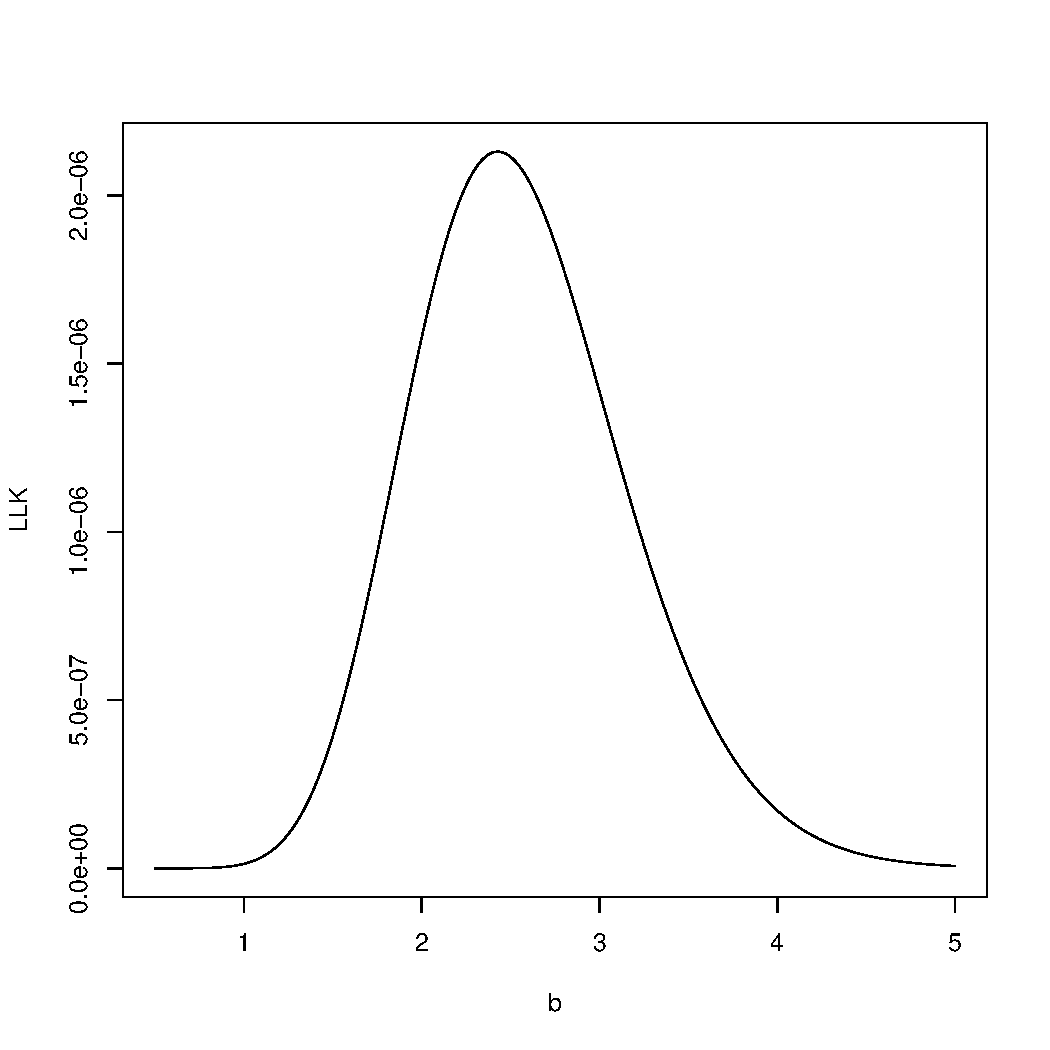
\includegraphics[width=0.8\textwidth]{Rplots.pdf}
\end{figure}
\newpage
\item This is the R code for finding the max value: \\
\begin{verbatim}
b = seq(0.5, 5, .01)
LLK = b^(17) * exp(-7 * b) / 69120
plot(b, LLK, type="l")
LK_max = max(LLK)
bmax = which(LLK == LK_max)
print(LK_max)
print(bmax)
MLE = b[bmax]
print(MLE)
\end{verbatim}
\item The numerical output was 2.43
\end{enumerate}
\end{document}